\documentclass[11pt]{sdm}
\usepackage{graphicx} % For figures
\usepackage{mathtools} % For smallmatrix envs
\usepackage{caption} % For figures captions
\usepackage{amsfonts} % For black board letters
\usepackage{bbm} % For black board 1
\usepackage[style=authoryear-comp, sorting=nyt, backend=biber]{biblatex} % For bibliography
\usepackage[acronym]{glossaries}
\addbibresource{Biblio.bib}

\newacronym{sca}{SCA}{Side-Channel Analysis}
\newacronym{scare}{SCARE}{Side-Channel Analysis for Reverse-Engineering}
\newacronym{spn}{SPN}{Substitution–Permutation Network}
\newacronym{aes}{AES}{Advanced Encryption Standard}

\makeatletter

\newrobustcmd*{\parentexttrack}[1]{%
    \begingroup
    \blx@blxinit
    \blx@setsfcodes
    \blx@bibopenparen#1\blx@bibcloseparen
    \endgroup
}

\AtEveryCite{%
    \let\parentext=\parentexttrack%
    \let\bibopenparen=\bibopenbracket%
    \let\bibcloseparen=\bibclosebracket
}

\makeatother

%numeroter les pages
\pagestyle{plain}

\title{SCARE for Hardware SPN}
\author{Paul \textsc{Saurou}}
\supervisorOne{Benoît \textsc{Gérard}}
\supervisorTwo{Margaux \textsc{Dugardin}}
\team{SDCyb1/EPOC/XCS}
%One of:
% ens-Rennes  esir    insa-rennes   rennes1  
% enssat    logoUbs   tsupelec
%here rennes1 for example
\school{supelec}


% the domain should be one or two of:
% Technology for Human Learning 
% Artificial Intelligence 
% Computer Arithmetic
% Hardware Architecture
% Automatic Control Engineering
% Bioinformatics 
% Biotechnology
% Computational Complexity 
% Computational Engineering, Finance, and Science
% Computational Geometry 
% Computation and Language 
% Cryptography and Security 
% Computer Vision and Pattern Recognition
% Computers and Society 
% Databases 
% Distributed, Parallel, and Cluster Computing 
% Digital Libraries
% Discrete Mathematics 
% Data Structures and Algorithms 
% Embedded Systems 
% Emerging Technologies 
% Formal Languages and Automata Theory 
% General Literature 
% Graphics 
% Computer Science and Game Theory 
% Human-Computer Interaction 
% Computer Aided Engineering 
% Medical Imaging 
% Information Retrieval 
% Information Theory 
% Ubiquitous Computing 
% Machine Learning
% Logic in Computer Science 
% Multiagent Systems 
% Mobile Computing
% Multimedia
% Modeling and Simulation 
% Mathematical Software 
% Numerical Analysis 
% Neural and Evolutionary Computing 
% Networking and Internet Architecture 
% Operating Systems 
% Performance 
% Programming Languages 
% Robotics 
% Operations Research
% Symbolic Computation 
% Sound
% Software Engineering 
% Social and Information Networks 
% Systems and Control 
% Image Processing 
% Signal and Image Processing 
% Document and Text Processing
% Web
\domain{Domain: Cryptography and Security}

%write your abstract here
\abstract{
    The confidentiality of modern cryptographic algorithms can either be proven mathematically or be based on difficult mathematical problems.
    However, these security proofs do not account for the particularities of the implementations.
    The algorithms are typically embedded in smart cards or run on a CPU, and attackers can retrieve secret information by observing and exploiting their physical leakages (e.g. power consumption).
    This type of attack is called \gls{sca}.
    Most often, the secret to recover is a private key while the details of the cryptographic system and its architecture are known.
    However, \gls{sca} can also be used to reverse engineer some parts or the whole structure of a cryptographic algorithm.
    This is called \gls{scare}.
    The purpose of this internship is to evaluate the potential threat of using \gls{scare} techniques on a hardware implementation of an \gls{spn} encryption scheme.
    In this bibliographic review, we introduce the context of the internship, as well as prospective issues and state-of-the-art \gls{scare} techniques on both software and hardware cryptographic systems.
}



\begin{document}
\maketitle

%*****************************************************************%

\section*{Introduction}

Cryptography is the study of techniques for secure communication in the presence of adversarial behavior.
It aims to guaranty confidentiality, integrity and authentication of a communication.
An encryption algorithm takes plaintext and key as input and outputs a ciphertext, that can be deciphered with another key to retrieve the plaintext.
For a symmetric algorithm, the encryption and the decryption keys are the same. 
The confidentiality property states that the ciphertext must be indistinguishable from a random stream of bytes for someone that does not know the secret decryption key.

The confidentiality of modern cryptographic algorithms can either be proven mathematically or be based on difficult mathematical problems.
However, these security proofs only apply to "black-box" adversaries, even if the algorithms are implemented in software or hardware modules.
These modules, such as smart cards or computer programs running on a CPU, are physically accessible, and attackers can retrieve secret information by observing and exploiting their physical leakages (e.g. power consumption).
This type of attack is called \acrfull{sca}.

Kerckhoffs stated that the security of a cryptographic device shall not rely on the secrecy of its mechanisms  \parencite{Kerckhoffs_1883}.
Following his principles, adversaries are supposed to have a perfect knowledge of the cryptographic algorithms.
Because of that, the secret to recover is generally limited to a private key while the details of the cryptographic system and its architecture are known to the adversary.
However, in some specific contexts, a secret implementation can add a layer of security, at least by increasing the practical difficulty of the attack.
For instance, a proprietary cipher can have its general structure revealed, but some constants kept secret.
The algorithm itself can be kept secret, or the details of its implementation.

\gls{sca} constitute a powerful tool to reverse-engineer some secret parts of a cryptographic implementation.
This is called \acrfull{scare} and it aims at recovering information about a cryptographic process (and not the manipulated data as usually targeted in side-channel attacks) based on the device power consumption.
It has been studied for software implementations of cryptography and can retrieve the characteristics of a proprietary algorithm quite efficiently. %TODO citations
However, few hardware implementations have been studied, and the existing literature is mainly targeted on Feistel ciphers.
Feistel ciphers are a very common category of symmetric cryptography algorithms.
The two most historically known Feistel ciphers are the US Data Encryption Standard (DES) and Blowfish. %TODO citation ?
Another very popular category of symmetric cryptography algorithms is \acrfull{spn}.
The most used \gls{spn} is the \acrfull{aes}. %TODO citation ?
The \gls{scare} possibilities for hardware \gls{spn} have almost not been studied yet, thus this internship aims at completing the \gls{scare} studies for \gls{spn}.

More specifically, the purpose of this internship is to evaluate the potential threat of using \gls{scare} techniques on a hardware implementation of an \gls{spn} encryption scheme.
To do that, a good understanding of existing side channel attacks on both software and hardware implementations is needed.
These attacks can be against \gls{spn} specifically or other similar symmetric cryptographic algorithms.
The goal is to propose new attack paths for the \gls{spn} hardware case and assess their relevance based on standardized benchmarks.
Both simulated data and real traces from a hardware capture board will be tested.
The different hypotheses and assumptions of each attack path will also be particularly looked upon.

In this bibliographic review, we first define the ciphers and the main \gls{sca} techniques that will be used later.
Secondly, we present an overview of \gls{scare} methods and their applications.
The analyses are separated depending on the cipher they target and their attacker model.
Thirdly, we focus on hardware implementations and explain the differences between software and hardware \gls{sca} and why there are fewer studies on hardware implementations.
We present the published hardware \gls{scare} attacks and show the lack of literature for \gls{spn} hardware \gls{scare}.
Finally, we discuss prospective issues and early reflections on the upcoming work in the conclusion.

%In this bibliographic review, we introduce the context of the internship, as well as prospective issues and state-of-the-art techniques on both software and hardware cryptographic systems.


\section{State of the art of Side-Channel Attacks}

Symmetric cryptography refers to the confidentiality protection of a communication between a sender and a receiver who share the same secret key.
Symmetric ciphers historically relied on legacy substitution ciphers but since the end of World War 2, stream and block ciphers are the norm.

In this section, we formally define the block ciphers we will be studying, in particular substitution–permutation network ciphers.
We also introduce some of the most classical and standardized implementations.
Then, we define several \acrlong{sca} state-of-the-art attacks on these implementations.
Finally, we present the most common countermeasures to \gls{sca}. 

\textbf{Substitution ciphers} replace the units of plaintext by ciphertext in a defined manner, with the help of a key.
Those are well known in history but can nowadays be easily decrypted using a frequency table or a similar mechanism.
They must not be mixed up with \acrlong{spn} that are a completely different kind of cipher.

\textbf{Stream ciphers} combine plaintext digits with a pseudo-random cipher digit stream called a keystream.

\textbf{Block ciphers} encrypt fixed-length blocks of plaintext.
Different modes of operation describe how to apply a block cipher to data larger than a block.
Block ciphers are the most widely used type of cipher.

This internship will focus on block ciphers, and especially on \acrlong{spn}.

\subsection{Block ciphers}

A block cipher consists of both an encryption function $E$ and a decryption function $D=E^{-1}$.
They both accept two inputs: a block of text of fixed size $n$ and a key of size $k$.
They output a block of size $n$.

The difference between different block ciphers is the definition of the function $E$ (and $D$).

Most block ciphers are iterated, which means that $E$ consists in the repetition of $r$ round functions $R_i$, where $i$ is the index of the round between $1$ and $r$.
The inputs of the function $R_i$ are a round key $K_i$ and the intermediate value $V_{i-1}$.
$V_i$ is the output of the previous round function.
The plaintext is $M=V_0$, the intermediate values are defined as following $ \forall i \in [ 1,r ] , V_i = R_i(V_{i-1},K_i) $ and the output $V_r = E(V_0) = E(M)$ is the ciphertext.
Another notation for the round function is $R_{K_i}(V_{i-1})$.

In most cipher designs, the round functions are chosen identical, except for the first and the last one.
Beginning or ending the cipher with easily reversible operations that do not depend on the key is useless so the first and last rounds are often simpler than the other rounds.

Choosing the number of rounds of an iterated block cipher scheme is a compromise between computing efficiency and cryptographic security.
Too few rounds allow for cryptographic attacks and too many rounds make the cipher less efficient.

We will now define two types of iterated block ciphers: Feistel network and \acrlong{spn}.

\subsubsection{Feistel ciphers}

In a Feistel scheme, the plaintext block is divided in two parts $(p,q)$ of equal length $n/2$.
The same round function $R$ is used for all rounds.
With the previous notations, it is $R: (p,q, K_i) \mapsto (q,p \bigoplus f(q,K_i))$ where $f$ is called the Feistel function.
Both the security and the performance of the Feistel network depend on the Feistel function $f$.
A specificity of Feistel schemes is that $f$ does not need to be invertible.
The decryption is almost identical to the encryption, the only difference being the reversal of the round keys order.
A sketch of a 3-rounds Feistel cipher is shown on Figure \ref{fig_feistel}

\begin{center}
    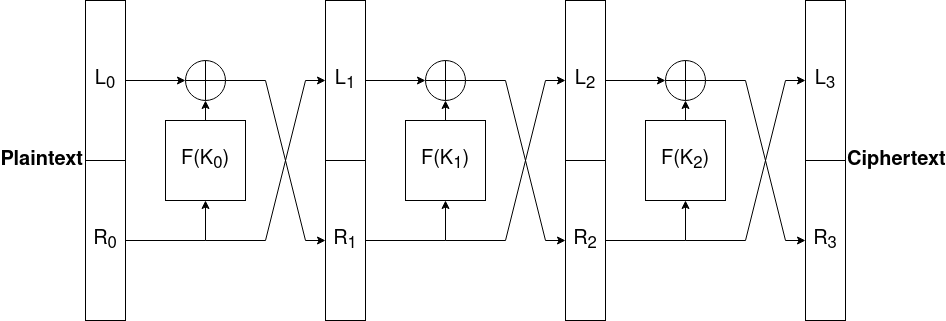
\includegraphics[width=1\textwidth]{../images/feistel.png}
    \captionsetup{hypcap=false}
    \captionof{figure}{A sketch of a Feistel network with 3 rounds, encrypting a plaintext $L_0+R_0$ into a ciphertext block $L_3+R_3$. The $L_i$ are the intermediate states and $F(K_i)$ is the Feistel function depending on the round key $K_i$.}
    \label{fig_feistel}
\end{center}
% TODO: add image ref in text


\textbf{The Data Encryption Standard (DES)} is a Feistel network scheme that has been highly influential in the advancement of cryptography.
It is unsecure due to its too short 56-bit key size which make it vulnerable to brute-force attacks.
Even if it is not used anymore, the DES design is technically interesting to study.
It consists in a 16 round Feistel network and operates on blocks of 64 bits.

First the 32-bit half-block is expanded to 48 bits using an expansion permutation function.
Then the 48-bit block is xored with the round subkey and goes through a substitution layer.
It is divided into eight 6-bit words which are replaced by 4-bit words using a lookup table.
Finally, the 32 outputs are mixed according to a fixed permutation.


\subsubsection{\gls{spn} ciphers}

In \acrfull{spn}, the round function consists of a xor with the round key, followed by a substitution stage and a permutation stage.
The intermediate state $V$ of size $n$ is xored with the round key and the result $V'$ is split into $l$ blocks $v'_1,v'_2,...,v'_l$ of equal length.
During the substitution stage, the intermediate state is mixed in some non-linear way.
It is based on a set of substitution-boxes (S-boxes) that substitute small block of bits (the input of the S-box) by another block of bits (the output of the S-box).
For the \gls{spn} to be reversible, the S-boxes have to be bijective.
The permutation stage rearranges all the bits of the output of the S-boxes each round, as shown on Figure \ref{fig_spn}.

More formally and with the previous notations, the round function is $R_{K_i} = \lambda \circ \gamma \circ \sigma_{K_i}$ with
\begin{itemize}
    \item $\sigma_{K}:V \mapsto V' = V \bigoplus K$ the key addition layer,
    \item $\gamma : V'=(v'_1,v'_2,...,v'_l) \mapsto V'' = S_1(v'_1),S_2(v'_2),...,S_l(v'_l)$ the substitution layer, where $(S_j)_{1\leq j \leq l}$ are non-linear substitution functions.
    \item $\lambda : V'' \mapsto A \times V''$ the linear layer, where $\times$ is the matrix product and $A$, an $l\times l$ matrix, is a parameter of the cipher.
\end{itemize}


The decryption is done by reversing the process.
It uses the inverses of the S-boxes and the permutations and apply the round keys in reversed order.

In some \gls{spn} implementations, the final round sometimes skips the linear layer and an additional key addition is often performed after the final substitution layer.

All the S-boxes do not have the same cryptographic properties.
% One is considered secure if it exhibits the avalanche effect, meaning that a small change in the input changes the output greatly. % Avalanche effect is for the linear part
One is considered secure if a small change in the input changes the output greatly.
For example, one input bit should change almost half of the output bits on average.
The S-boxes $(S_j)_{1\leq j \leq l}$ can be chosen identical to ease the implementation and assure that one is not weaker than the others.

\begin{center}
    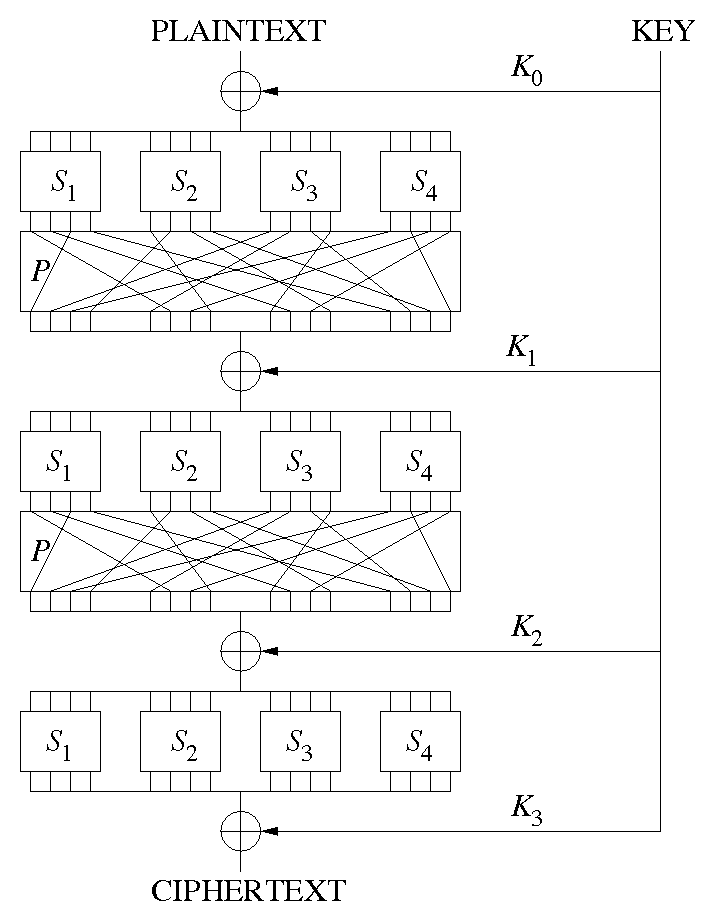
\includegraphics[width=1\textwidth]{../images/spn_wiki.png}
    \captionsetup{hypcap=false}
    \captionof{figure}{A sketch of a \acrlong{spn} with 3 rounds, encrypting a plaintext block of 16 bits into a ciphertext block of 16 bits. The S-boxes are the $S_i$, and the round keys are the $K_i$.}
    \label{fig_spn}
\end{center}
% TODO: change figure and caption (or add P box in text)

\textbf{The \acrfull{aes}} is the replacement of DES chosen by the NIST in 2001.
The algorithm is a specification of the Rijndael design.
It is an \gls{spn} that exists in three variants:
\begin{itemize}
    \item 10 rounds and 128-bit keys,
    \item 12 rounds and 192-bit keys,
    \item 14 rounds and 256-bit keys.
\end{itemize}

The 128-bit block plaintext is arranged in a 4$\times$4 byte matrix, as shown in figure \ref{fig_aes}.
% $\begin{psmallmatrix}
%     m0 & m4 & m8 & m12 \\
%     m1 & m5 & m9 & m13 \\
%     m2 & m6 & m10 & m14 \\
%     m3 & m7 & m11 & m15
% \end{psmallmatrix}$
The round keys are derived using the \gls{aes} key schedule.
All the 16 S-boxes are the same, and their design is chosen to have no fixed points.
The substitution operation is often referred as SubBytes operation.
The linear layer is divided into a ShiftRows and a MixColumns operations.
The ShiftRows step cyclically shifts the bytes in each row by a certain offset (from 0 to 3).
% $\begin{psmallmatrix}
%     m0 & m4 & m8 & m12 \\
%     m1 & m5 & m9 & m13 \\
%     m2 & m6 & m10 & m14 \\
%     m3 & m7 & m11 & m15
% \end{psmallmatrix}
% \rightarrow
% \begin{psmallmatrix}
%     m0 & m4 & m8 & m12 \\
%     m5 & m9 & m13 & m1 \\
%     m10 & m14 & m2 & m6 \\
%     m15 & m3 & m7 & m11 \\
% \end{psmallmatrix}$


The MixColumns step then multiplies each column in place by a standard matrix.
% $\begin{psmallmatrix}
%     2 & 3 & 1 & 1 \\
%     1 & 2 & 3 & 1 \\
%     1 & 1 & 2 & 3 \\
%     3 & 1 & 1 & 2
% \end{psmallmatrix}$
During this step, each byte of the column influences all the four bytes of the output.

\begin{center}
    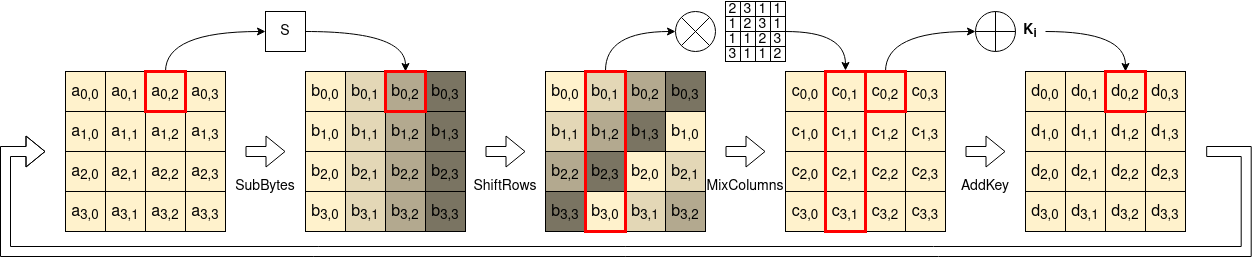
\includegraphics[width=1\textwidth]{../images/aes2.png}
    \captionsetup{hypcap=false}
    \captionof{figure}{A sketch of a round of \gls{aes}. S is the S-box and $K_i$ the round key.}
    \label{fig_aes}
\end{center}

The details of the \gls{aes} standard are defined in the Federal Information Processing Standards Publication 197 (FIPS PUBS 197) \parencite{Standards2001}.

\subsection{\acrlong{sca} state-of-the-art attacks}

All the implementations of cryptographic algorithms in real world devices provide more information to an attacker than just the plaintext and the ciphertext.
These side-channel leakages can consist in the timing of operations, power consumption, electromagnetic emanations, etc.
An attacker can observe these leakages.
However, such observations might require direct access to the cryptographic module or complex experiments with precise probes placement or capture boards.
These leakages are not taken into account by the mathematical models and very little side-channel information is enough to break common ciphers that are proven safe against an attacker who can only access the inputs and the outputs.
The \gls{sca} attacks, also called passive attacks and their corresponding countermeasures have been studied extensively over the past decades.

In the following, side channel attacks consist in associating the power consumption of a cryptographic module with the data processed by the module at the same time.
Indeed, the physical properties of semiconductors link the data processed by a chip to its power consumption.

\textbf{Single power analysis} (SPA) involves directly interpreting power consumption measurements collected during cryptographic operations \parencite{Kocher_Jaffe_Jun_1999}.
SPA can yield information about a device's operation as well as key material.
It does not use a leakage model as it is a very simple analysis.

For all the other \gls{sca}, side channel leakages are assumed to follow a leakage model.
This leakage model can either be profiled or non-profiled.
The choice of a model depends on the system under study and its leakages.
As it is a strong assumption to make, a wrong leakage model may not lead to a successful attack.

\subsubsection{Profiling attacks}

Profiling attacks assume that the attacker has access to a clone device to model its leaking behavior.
Attacks using such a model can retrieve a secret key with just a few traces but often need a lot of training on a specific architecture.

\textbf{Template attacks} create a profile of the attacked device with many generated traces and use it to later find the secret of the victim with a very small number of traces.

First described in 2003, it uses a copy of the protected device to record numerous power traces using many plaintexts and keys \parencite{Chari_Rao_Rohatgi_2003}.
The noise is modeled using multivariate Gaussian distributions, one for each possible subkey.
If a subkey is a byte, then the attack would need 256 different templates.
The samples are used to identify the points where the differences between averaged signals are the largest.
These are points of interest and the model will only focus on their values.
The "templates" are then created for each subkey on these points of interest by combining the mean signal $M_i$ and the noise covariance matrix $\Sigma_{N_i}$.
The attack then consists in computing the probability that the trace from the target device originates from each template.
Selecting the highest probability is optimal.
Depending on the training set, a few leakages can be enough to identify a subkey.
The authors also calculate the error probability of their test and explain how to improve the attack by pruning the least probable hypotheses.


Over the last years, \textbf{Deep Learning based Attacks} (DL) have reached the state of the art of side channel attacks.
The training phase builds a profiled model that is very efficient against one architecture and one leakage type.
Deep Neural Networks (DNNs) are able to efficiently break implementations of \gls{aes} that resisted to other types of \gls{sca}, particularly when desynchronization occurs \parencite{Maghrebi_Portigliatti_Prouff_2016}.
% TODO: explain how DNNs are useful. Or not and just conclude

\subsubsection{Non-profiled attacks}

Non-profiled attacks use non-profiled models that suppose a link between the data processed and the corresponding leakages.
They are more general than profiled models because they are not restrained to one specific implementation.
To model the link between data transitions and power consumption, the Hamming weight and Hamming distance models are often used.
We first present these two models, then the attack that use them.
Finally, we describe the Mutual Information Attack (MIA), which is based on its own model.

\paragraph{}
The \textbf{Hamming Distance} of $a \in \mathbb{F}_2^n$ and $b \in \mathbb{F}_2^n$ is $H(a \bigoplus b) = \sum_{i=0}^{n-1} \mathbbm{1}_{a_i \neq b_i}$ where $a_i$ (resp. $b_i$) is the $i$th bit of $a$ (resp. $b$).
It counts the number of transitions when $a \rightarrow b$.
For consecutive values in the same register, this metric correlates the Hamming distance with the power consumption.
However, the attacker needs to obtain consecutive data values to use this model.
A simpler solution is to consider that $a=0$. The model then becomes the following.

The \textbf{Hamming Weight} of $a \in \mathbb{F}_2^n$ is $H(a) = \sum_{i=0}^{n-1} \mathbbm{1}_{a_i = 1}$ where $a_i$ is the $i$th bit of $a$.
It counts the number of bits set to 1 when storing the variable $a$.
It is the most widely used leakage model, because it is simple and efficient to model the leakages of software implementations, whereas the Hamming distance model is better for hardware implementations.

\paragraph{}
\textbf{Differential Power Analysis} (DPA) involves statistical tools to study multiple power consumption leakages from a cryptographic module.
It aims to remove noise by using signal processing and error corrections techniques.
The analysis assumes a non-profiled leakage model.

\smallbreak
\textbf{Correlation Power Analysis} (CPA) is a kind of DPA but makes further assumptions.
It supposes a power consumption model, most often the Hamming weight model or the Hamming distance model.
It then tries to correlate the modeled power consumption with the real consumption using the Pearson correlation coefficient. % TODO: Maybe explain what the PCC is (or not)

\smallbreak
\textbf{Mutual Information Attacks} (MIA) uses entropy and mutual information between the leakage and the predicted data.
Thus, it does not rely on the Hamming distance or Hamming weight models.
This model does not require any previous knowledge of the studied device and can be applied in any context.
Prouff and Rivain present a theoretical analysis of the assumptions made in side channel attacks \parencite{Prouff_Rivain_2009}.
MIA is studied in the Gaussian leakage model and in the case of masked implementations.
By making fewer assumptions about the model, MIA has worse performance than other techniques using correlations between traces on devices following the Hamming weight model.
However, it could retrieve the key in a context where the trace is not linearly linked to the Hamming weight of the manipulated data.

\paragraph{}
These \gls{sca} aim to retrieve the key, or some other secret component, involved in a known algorithm.
Template attacks even use a replica of the attacked device to "prepare" the attacks.

There are many countermeasures to prevent these attacks or make them more difficult.
The following subsection is about the main \acrlong{sca} countermeasures.

\subsection{\acrlong{sca} countermeasures}

There are two types of \gls{sca} countermeasures. 
The first one consists in eliminating or reducing the leakages and the second one consists in making the leaked information unrelated to the secret data.

Physical shielding, power line conditioning, noise addition and adding random delays are of the first type.
They do not prevent \gls{sca} but with these countermeasures activated, an attacker has to collect more measurements.

Masking is an effective countermeasure of the second type.
It consists in decorrelating the intermediate results from the secret values.
To do that, a different random value is used each round and the operations are modified so that the final result does not depend on the secret value anymore.
Implementing masking effectively is very specific to each architecture and each attacker model.
The most common masking strategies are boolean (xor $\bigoplus$) and arithmetic (+ mod $2^n$). % TODO: choose a reference for masking


These are the main side channel analysis techniques and countermeasures. 
Nonetheless, it is also important to verify the security of cryptographic implementations against weaker opponents that do not know the exact implementation or its details.
For cryptographic systems that choose to use proprietary algorithms or a specific set of parameters for a known standard, the architecture itself is a secret component that can be determined through \gls{sca}.
The following section is about \acrlong{scare} and aims at assessing the gains or losses in security of choosing secret parameters for symmetric cryptography algorithms.


% \parencite{Chari_Rao_Rohatgi_2003} presents template attacks, "the strongest form of side channel attack possible in an information theoretic sense".

% \parencite{Prouff_Rivain_2009} presents the theory of Mutual Information Attacks (MIA) in side channels.

% Machine Learning is very popular right now. Thesis of \parencite{Masure}

\section{\acrlong{scare}}

\acrfull{scare} uses side-channel information to reverse-engineer the secret parts of a cryptographic implementation.
It applies the techniques of \gls{sca} to recover implementations details among:
\begin{itemize}
    \item secret constants such as the S-boxes of a \gls{spn} \parencite{Novak_2003},
    \item algorithmic structure such as the number of rounds or the size of the S-boxes used,
    \item which technologies and methods are used by the developer of the products.
\end{itemize}

\subsection{\gls{scare} attacks on non \gls{aes} ciphers}
\label{scare_non_aes}

\subsubsection{\gls{scare} of the GSM}
The first \gls{scare} attack was proposed by Novak in 2003 to retrieve the secret authentication and session key generation algorithm of the GSM standard \parencite{Novak_2003}.

The COMP128-2 algorithm used in SIM cards was kept secret despite Kerckhoffs' principle.
Knowing the architecture, the computations involved and the secret key, Novak retrieves the contents of substitution blocks implemented as lookup tables by analyzing the power consumption of the cipher.

The idea behind the attack is to use \textbf{collision analysis}.
It assumes that the same value of an input leads to similar leaks of the considered operation.
Identifying equal intermediate results allows an attacker to restore the content of the lookup table and thus break the substitution block.

To do that, it uses the means of measurements for all the possible values of a given input byte to distinguish them.
The equality between the leakages provides a set of equations at each round of the cipher.
Combining these sets of equations allows to solve them and recover the lookup table content.

This attack is based on the assumption that two lookups to the same value gives very similar leakages.
It relies a lot on the quality of the leakages to identify identical lookups.
Because of that, table masking is an effective countermeasure.


\subsubsection{\gls{scare} of the DES}
\label{scare_des}

Another \gls{scare} method relies on \textbf{correlation power analysis}.
An example of such attack is the reverse engineering of DES, in which the authors assume that the structure and the constants are unknown \parencite{Daudigny_Ledig_Muller_Valette_2005}.
Strong assumptions on the quality of the power leakages allow the attacker to extract scheduling information for each bit at the clock cycle level using CPA.
It means that the attacker knows exactly when each bit is manipulated.
This scheduling information from the power consumption allows the attacker to recover a good deal of information from the software implementation of DES.

Identifying patterns in power consumption and scheduling information allow to recover the general structure of the cipher: number of rounds, use of xor operation and table lookups.
For example, groups of bits manipulated together often correspond to S-box inputs.
Removing the noise and observing the scheduling information of the first round input of DES allows to recover the content of the DES expansion table line by line.
The same thing can be done for the following S-box layer and the permutation table.
The key scheduling algorithm can also be found using the same technique.

The scheduling information can then be used to isolate traces corresponding to each S-box and perform another \gls{sca} attack to recover the key.


\textbf{CPA} techniques for reverse engineering can also be used under much weaker assumptions.
Another attack is possible in the known plaintext or ciphertext attacker model \parencite{Guilley_Sauvage_Micolod_Réal_Valette_2010}.
It retrieves the S-boxes of a modified DES using custom S-boxes by using brute force.
To attack $i$ input bits of an S-box, the attacker only considers a set of traces that keep $6-i$ bits of the target S-box to a constant value (which is possible since the plaintext is chosen).
A correlation analysis then recovers the partial function that maps the $i$ input bits that are modified to one output bit.
Repeating this operation for all output bits and all group of input bits unravel the whole S-box design.
To recover one S-box of DES, 960 CPAs are necessary using this method on 2 input bits at a time.


%\parencite{Novak_2003} presents a side-channel attack on substitution blocks with a demonstration on a SIM card using COMP-128 cipher.

%\parencite{Daudigny_Ledig_Muller_Valette_2005} presents a SCARE attack on DES and propose new methods to exploit the power measurement information.

%\parencite{Guilley_Sauvage_Micolod_Réal_Valette_20DES10} presents two SCARE attacks on the parameters of a LFSR and DES.

\subsection{\gls{scare} attacks on \gls{aes}-like ciphers}

The \acrlong{aes} is a publicly-known and clearly defined architecture. 
However, its parameter values can be changed to obtain a new cipher, that is not \gls{aes} but has the same structure.
% Following Kerckhoffs' principle, this new cipher may not be safer than a classic implementation of AES.
The following examples show how the secret parameters can be recovered using \gls{scare}.

\subsubsection{\gls{scare} of \gls{spn}}
\label{scare_of_spns}

This \gls{scare} method is designed for all \gls{spn} structures, including modified \gls{aes} ciphers \parencite{Rivain_Roche_2013}.
It considers that the attacker can select parts of the side-channel traces where the S-box computations are located.
The attacker must be able to decide on collisions between the processed values from the observation of these traces.
For that, any \gls{sca} method can be used.
The attacker also knows the plaintext.
If the plaintext is chosen, the complexity of the attack is lowered.

Then the attack consists in building simple linear equations systems to recover the S-box values, the linear layer coefficients and the secret round keys.
It retrieves the first round key by fixing its first bit and then identifying the collisions between the already known bits and the remaining bits.
Knowing the first secret round key, the collisions happening before and after the 2nd round allow to build a system of linear equations involving the linear layer, the S-box and the second secret round key.
Given enough traces, the system can be solved.
Then, only the remaining round keys are left to be discovered.
It can be done using the same method as for the first one.

This attack is very generic and can be applied to all \gls{spn} schemes.
It also works if the leakage is noisy.

According to the authors, a sufficient countermeasure is to combine masking and operation shuffling.
Non-sequential execution is also outside the scope of the attack and make it inefficient.


\subsubsection{\gls{scare} of masked \gls{aes}}

This very general attack on \gls{spn} has been refined for \gls{aes} in 2015 under more restrictive assumptions \parencite{Clavier_Isorez_Marion_Wurcker_2015}.
The work is divided in two parts.

The first one does a \gls{scare} of the \gls{aes} under a very similar model than the one presented in section \ref{scare_of_spns}.
It still considers that the attacker can identify collisions between two different S-Box computations.
The difference is that this method can deal with masking and operation shuffling at the cost of only applying to \gls{aes} with secret parameters.
In particular, the S-box has to be the same for each round and the key derivation algorithm must be the one from \gls{aes} with secret constants.

The second part does a \gls{scare} of the \gls{aes} assuming that the attacker can identify collisions of Hamming weights of inputs/outputs of different S-box computations.
This model is weaker but more realistic.
It can also be adapted to evade simple masking.

\paragraph{}
Clavier et al. first consider an 8-bit Boolean masking that only refreshes the randomization of S-boxes at each execution because of time and memory constraints.
It is a common way to implement masking without it being too expensive.
To address the masking countermeasure, they use the intra-traces setting, meaning that the attacker is able to detect collisions between two S-Box only in the same execution.
Then collisions that happen during one execution can be exploited.
Masking on other operations do not affect the attack.

The shuffling countermeasure is more complex to evade.
It shuffles the 16 bytes S-box computations at each round, causing the collisions' observation to no longer give information about the index of the input bytes.
The remaining information is the number of different S-Box inputs at each round, and their number of occurrences.
To retrieve the first round key, it finds a plaintext such that the first round SubBytes operation only presents one colliding value occurring more than once.
By modifying each one of the 16 bytes of the plaintext and picking the indexes for which the multiplicity of the colliding value is reduced, the attacker can infer relations between the key bytes.
The process can be repeated with new plaintexts until enough relations are obtained, and the first round key can be determined (up to a xor with a constant).
The same can be done for the last round key.

To recover the S-box, the same concept is used.
Repeated collisions between the first S-box and the last S-box computations are identified and analyzed.
Each collision gives information about the values of a small group of bytes and repeating the operation for multiple chosen plaintexts eventually gives enough information to retrieve the S-box content.

Since the first and last round keys are known, the key scheduling algorithm can be found through exhaustive search.
To recover the ShiftRows and MixColumns parameters, the attacker can craft plaintexts by only changing one byte to obtain a small subset of possible values for MixColumns columns and ShiftRows parameters.
Different byte values provide new sets of possible values and their intersection reveals the secret parameters.
All the secret parameters of the \gls{aes} implementation have then been discovered.

\paragraph{}
To perform their second \gls{scare} attack on a modified \gls{aes} under the Hamming weight model, Clavier et al. introduce and reason on special sets.
They are constituted of the inputs (respectively the outputs) that have a given Hamming weight and whose S-box output (respectively input) has another given Hamming weight that will collide under the Hamming weight collisions model.
The attack first retrieves the first and last round keys and the ShiftRows parameters, then builds the special sets by analyzing collisions and non-collisions between chosen plaintexts, and reasons on their cardinal.
The special sets allow to reduce the number of potential candidates for each byte value during the MixColumns and S-box retrieval stages.
If a set has a cardinal of 1, then it identifies one unique value.
This attack is very efficient on a simulated implementation and can recover the parameters of an \gls{aes} using approximately 250 traces, whereas 400 (respectively 4000) are needed under the unprotected (respectively protected by a first-order Boolean masking and a random shuffling of operations) collision value model.


% Est-ce vraimentpertinent de parlerShiftRow d'une cryptanalyse dans un rapport sur les SCA ?
%\parencite{Tiessen_Knudsen_Kölbl_Lauridsen_2015} presents an integral cryptanalysis of an AES with a secret S-box and fewer rounds. It is not a SCA but is still closely related to our subject.

%\parencite{Rivain_Roche_2013} presents a generic SCARE attack against a wide class of SPN block ciphers.

%FIRE (injection fault attempts) and SCARE attacks to recover the full set of secret parameters of an AES-like software implementation, even with masking and shuffling \parencite{Clavier_Isorez_Marion_Wurcker_2015}.

\section{Application to hardware implementations}

\subsection{Differences between software and hardware cryptographic implementations}

Software implementations are exposed to illegitimate access to their machine code through memory dumping.
This can often be done without damaging the component.
Because of that, it is more secure to implement the cryptographic algorithm into a specific device.
It allows for better performances and better security through isolation of the component.

Also, implementing cryptography in hardware modules makes it more difficult to use \gls{sca} techniques.
Indeed, many \gls{sca} attacks assume that the execution is sequential, whereas cryptographic modules implemented on an ASIC or an FPGA use parallelization whenever it is possible.
Parallelizing the S-box lookups makes collisions based attacks impossible and increases the measurements needed for the other attacks.
Then, hardware cryptographic implementations leakages are noisier, due to the physical setup and can use other countermeasures, such as desynchronized execution.
So attacks on hardware devices cannot recover as much information as attacks on software algorithms.
For example, the precise scheduling information recovered in the attack presented in \ref{scare_non_aes} is unrealistic on a hardware target \parencite{Daudigny_Ledig_Muller_Valette_2005}.


Due to the higher cost of developing, evaluating and attacking hardware cryptographic implementations, and the lack of reproducibility of the studies due to different experimental setups (acquisition platform sensitivity, cryptographic algorithm implementation, board's noise), the literature on the subject is scarcer.

To address the lack of uniformized benchmark, the DPA Contest v2 proposed in 2010 a common framework for multiple team to compare their attacks \parencite{Clavier_Danger_Duc_Elaabid_Gérard_Guilley_Heuser_Kasper_Li_Lomné_et_al_2014}.
The target is an FPGA implementation of an \acrshort{aes}-128, and it considers known-message and profiled attacks.
The acquisition board and its setup are precisely defined, and many metrics are used to evaluate the attacks: partial success rate, partial guessing entropy, global success rate, execution time and memory footprint.

The results of the contest emphasize many differences between software side channel analysis and hardware side channel analysis.
An example is the higher inaccuracy of the models such as the Hamming distance model used to approximate the traces.
This inaccuracy makes classical attacks adaptation more difficult but also allows new opportunities of improve them.

% \begin{itemize}
%     \item The sequential execution becomes parallel
%     \item There is even more noise
%     \item SCA leaks cannot be determined as precisely
%     \item It takes more time to implement, develop and attack
% \end{itemize}

% \parencite{Clavier_Danger_Duc_Elaabid_Gérard_Guilley_Heuser_Kasper_Li_Lomné_et_al_2014} presents the result of the DPA contest.

\subsection{\gls{scare} on hardware design}

The \gls{scare} attacks on hardware design mostly focus Feistel networks.

An attack targeting a general Feistel design was presented in 2008 \parencite{Réal_Dubois_Guilloux_Valette_Drissi_2008}.
The experiments of this attack use electromagnetic radiations instead of the power consumption as side channel leakage.
Measuring electromagnetic radiations allows to detect the register state changes as in the power consumption model.
With more experimental difficulties, the electromagnetic probes can observe the current at the register level.

The attacker model of this reverse engineering is a chosen plaintext scenario and the attacker can only measure the global system leakages.

To identify a Feistel scheme, a CPA mean on the left part of the plaintext contains one peak and on the right part it contains two peaks.
Indeed, the right part of the plaintext is used in both the first and second rounds, whereas the left one is only used once.
The number of rounds of a ciphering operation can be identified by analyzing the peaks in the electromagnetic radiation.

To guess the Feistel function, the attacker fixes the right part of the plaintext and modifies its left part.
It recovers the output of the Feistel function 4 bits by 4 bits by doing a CPA on the first round of the Feistel network.
For each 4-bits input word, the CPA gives away the output of the Feistel function.
The attacker can use the same technique to recover the rest of the Feistel function.
If the level of noise is sufficiently low, the attacker can even do it bit by bit instead of four bits by four bits.

To recover the whole Feistel function in the general case, it is considered as a vector function made of polynomials of the inputs bits and of degree $d$.
If $n$ is the size of the input/output, there are around $n^d/d!$ coefficients for each one of the $n$ polynomials and as many \gls{sca} to perform.
However, commonly used schemes are more restrictive and thus reduce the number of possibilities to account for.

The proposed optimization considers a Feistel function built by concatenating a random function and a linear compression that reduces the number of bits.
This strong assumption reduces the number of input/output pairs needed to reverse engineer the Feistel function to $2^d + (n-d)d$, where the linear compression is from $n$ bits to $d$ bits.
The improvement makes the attack much more feasible in practice. 


In 2010, Guilley et al. presented a \gls{scare} of a DES implemented on FPGA \parencite{Guilley_Sauvage_Micolod_Réal_Valette_2010}.
We already went into the details in Section \ref{scare_des}.
The concept behind this attack is similar to the one presented just before \parencite{Réal_Dubois_Guilloux_Valette_Drissi_2008}.
In a nutshell, Guilley et al. retrieve the S-boxes of a modified DES using custom S-boxes by performing CPAs and recollecting the S-box content 2 bits by 2 bits.

%\parencite{Réal_Dubois_Guilloux_Valette_Drissi_2008} presents a SCARE attack on a general Feistel scheme with an hardware design.

% SAKURA board reference

% \parencite{Guilley_Sauvage_Micolod_Réal_Valette_2010} presents two SCARE attacks on the parameters of a LFSR and DES, implemented on FPGAs.

% SCA attacks on FPGAs (\parencite{Peeters_Standaert_Donckers_Quisquater_2005} or more relevantly \parencite{Standaert_Ors_Preneel_2004} or something more recent)


\section{Conclusion}

This bibliographic report presents a comprehensive overview of block ciphers, \gls{sca} techniques, and \gls{scare} methods and highlights the need for further research in this area.
The studies analyzed provide a synthesis of \gls{sca}, including the methods used, leakage models, assumptions made, and countermeasures proposed.

The implementation of cryptographic algorithms on hardware presents more difficulties for \gls{sca} due to experimental issues, leading to noisier leakages.
Also, because of the parallel execution on hardware modules, collisions attacks are not possible anymore.
This type of \gls{sca} is very efficient on sequential software cryptographic implementations but cannot be applied on hardware.

Comparing two \gls{sca} studies is challenging because of the variation in attacker and leakage models.  
Efforts have been made to standardize hardware \gls{sca} benchmarks, as demonstrated in the DPA contest \parencite{Clavier_Danger_Duc_Elaabid_Gérard_Guilley_Heuser_Kasper_Li_Lomné_et_al_2014}.
Today, many studies on FPGAs use the same SASEBO capture board \parencite{Satoh}.

The application of \gls{sca} to reverse engineering is a more recent development and encompasses a wide range of scenarios, from partial recovery of parameters in known architectures to uncovering all aspects of an unknown cipher.
Most of the \gls{scare} literature focus on software, and the existing literature on hardware is mainly targeted on Feistel ciphers.
This internship aims to address this gap by evaluating the potential threat of \gls{scare} on a hardware implementation of an \gls{spn} encryption scheme.
This \gls{spn} is a tuned \gls{aes} cipher implemented on a dedicated \gls{sca} board known as SASEBO-GIII.
Theoretical attack paths will be proposed and tested on a simulated cipher, followed by a practical component.
It involves using the SASEBO-GIII capture board to obtain power consumption leakages and clean the hardware signals, followed by testing and adapting the theoretical attack paths to real traces.
Special attention will be paid to explaining the impacts of the attacker model assumptions on the \gls{scare} attack.



% SAKURA board reference


\printbibliography[title=Bibliographie]

\end{document}
%%% Local Variables:
%%% mode: latex
%%% TeX-master: t
%%% End: